\PassOptionsToPackage{unicode=true}{hyperref} % options for packages loaded elsewhere
\PassOptionsToPackage{hyphens}{url}
%
\documentclass{book}        % from not too short p76 pagestyle
%\usepackage{fancyhdr}
%\pagestyle{fancy}
%ensure chapter section headngs in lower case
%
\usepackage{graphicx}
\DeclareGraphicsExtensions{.png,.jpg}
\usepackage{xeCJK}
\setCJKmainfont{SimSun}
\usepackage{lmodern}
\usepackage{amssymb,amsmath}
\usepackage{ifxetex,ifluatex}
\usepackage{fixltx2e} % provides \textsubscript
\ifnum 0\ifxetex 1\fi\ifluatex 1\fi=0 % if pdftex
  \usepackage[T1]{fontenc}
  \usepackage[utf8]{inputenc}
  \usepackage{textcomp} % provides euro and other symbols
\else % if luatex or xelatex
  \usepackage{unicode-math}
  \defaultfontfeatures{Ligatures=TeX,Scale=MatchLowercase}
\fi
% use upquote if available, for straight quotes in verbatim environments
\IfFileExists{upquote.sty}{\usepackage{upquote}}{}
% use microtype if available
\IfFileExists{microtype.sty}{%
\usepackage[]{microtype}
\UseMicrotypeSet[protrusion]{basicmath} % disable protrusion for tt fonts
}{}
\IfFileExists{parskip.sty}{%
\usepackage{parskip}
}{% else
\setlength{\parindent}{0pt}
\setlength{\parskip}{6pt plus 2pt minus 1pt}
}
\usepackage{hyperref}
\hypersetup{
            pdfborder={0 0 0},
            breaklinks=true}
\urlstyle{same}  % don't use monospace font for urls
\usepackage{longtable,booktabs}
% Fix footnotes in tables (requires footnote package)
\usepackage{multirow} %for tabular combine multirow
\IfFileExists{footnote.sty}{\usepackage{footnote}\makesavenoteenv{longtable}}{}
\setlength{\emergencystretch}{3em}  % prevent overfull lines
\providecommand{\tightlist}{%
  \setlength{\itemsep}{0pt}\setlength{\parskip}{0pt}}
\setcounter{secnumdepth}{0}
% Redefines (sub)paragraphs to behave more like sections
\ifx\paragraph\undefined\else
\let\oldparagraph\paragraph
\renewcommand{\paragraph}[1]{\oldparagraph{#1}\mbox{}}
\fi
\ifx\subparagraph\undefined\else
\let\oldsubparagraph\subparagraph
\renewcommand{\subparagraph}[1]{\oldsubparagraph{#1}\mbox{}}
\fi

% set default figure placement to htbp
\makeatletter
\def\fps@figure{htbp}
\makeatother
\date{}

\usepackage{graphicx}

\raggedbottom


\begin{document}


\begin{titlepage}\thispagestyle{empty} \vspace*{3em}
%\includegraphics[width=13cm]{aBookCover2latexScreenshot2023-03-08130046.jpg}
\clearpage\newpage \thispagestyle{empty} \mbox{} \cleardoublepage

%\thispagestyle{empty} \vspace*{7em}{\centering\Huge  管理A++  \par}{\centering -- 从个人提升到 以数据说话 \par}\cleardoublepage

\thispagestyle{empty} \vspace*{7em}{\centering\Huge 管理A++  \par}

\thispagestyle{empty} \vspace*{\fill} \parbox{.8\textwidth}{\raggedright \scriptsize
\textit{impossible} publisher 2022

printed blindfolded

design: \LaTeX
}
\end{titlepage}
\clearpage \thispagestyle{empty}\cleardoublepage
\newpage % Make sure the following content is on a new page

%----------------------------------------------------------------------------------------
%	TABLE OF CONTENTS
%----------------------------------------------------------------------------------------

\tableofcontents % Prints the table of contents

%----------------------------------------------------------------------------------------
%	INTRODUCTION SECTION
%----------------------------------------------------------------------------------------

%\includeonly(filename,filrname,.......)




\chapter{A0 序 感谢 前言} % Introduction chapter suppressed from the table of contents

\hypertarget{ux5e8f-preface}{%
\section{序 Preface}\label{ux5e8f-preface}}

\hypertarget{ux524dux8a00-prologue}{%
\section{前言 Prologue}\label{ux524dux8a00-prologue}}

"There are no hard distinctions between what is real and what is unreal,
nor between what is true and what is false. A thing is not necessarily
either true or false; it can be both true and false."

\begin{description}
\item[]
\begin{description}
\tightlist
\item[]
Harold Pinter , 1958
\end{description}
\end{description}

我是从自学社会系统理论 (socio-technical systems theory) 开始听到 Russell
Ackoff 的名字。
开始关注他的著作是从看完他的演讲视频开始：觉得他演讲很清晰，针对主题用实例解释，而且观点都很精炼，并且不落书套，已经经过深思熟虑的结果。我便开始搜索他简历与著作：

原来在70至80年代，他在宾州大学 (U. of Pennsylvania) 沃顿 (Wharton
School) 举办 Social Systems Science Program
课程，帮助学生学习与研究社会系统。这课程被后人评价：``能集合理论与实际，帮助学员能把学到的用于自己熟识的领域。''

他出版了超过40本书，除了第一本《运筹学》(Operations
Research，1957)外，其他大部分都与社会系统或管理相关。

2007年，他 Herbert J. Addison 与 Sally Bibb 出版 "Management f-Laws :
How organizations really
work"：（也是他的最后一本书）。当我在图书馆里找到这本很薄的小书，发现与他之前出版的书很不同：

\begin{itemize}
\tightlist
\item
  风格轻松，之前的书，都是偏学术性，以学者的口吻写，这小书就显得幽默
\item
  简单易读：里面简单每2页介绍一条，共81条 f-laws.
\end{itemize}

他解释说： ``f-laws are truths about organizations that we might wish to
deny or ignore -- simple and more reliable guides to managers' everyday
behavior than the complex truths proposed by scientists, economists,
sociologists, politicians and philosophers.''

但这小书也有不足：每一条右边一页都是 Sally Bibb
的反馈意见，但都是基于她自己的想法，缺乏实例，有些更只是用另一个角度把左边A的点重新说。

所以我便基于古人写《左传》（注）的方式，依据 Ackoff
教授每条经典道理，加上我自己的经历或咨询过企业的故事，希望能帮助读者能更好理解他每条的重点。

我写《敏捷开发A++
实践》时，曾经收到反馈说有些章太长（十几页），如能压缩可以提升易读性，所以在这小册里，把每条的相关故事都控制在一页内。

基于Ackoff
教授的XX条基础，我后面继续尝试其他管理大师，如XXX，也写出f-laws，所以这小册取名为《管理
A++》。

正如英国剧本作家Harold
Pinter说，任何事情没有绝对的对或错，因为各企业或团队的环境、能力不同，这小册里的道理不一定都适用。只希望站在巨人的肩膀上，借用实例，让读者更了解道理背后的原意，并得到启发。

\begin{description}
\tightlist
\item[]
注：《春秋》是孔子根據魯國史官所編之史書重新修訂而成，記述從魯隱公元年（公元前722年）到魯哀公十四年（公元前481年）間二百四十二年之歷史。但《春秋》文字过于简质，后人不易理解，所以相继各种解释和说明，称之为``传''，例如《公羊传》，其中《左传》主要以写故事的方式来解读《春秋》，
\end{description}

\hypertarget{ux53c2ux8003-references}{%
\section{参考 References}\label{ux53c2ux8003-references}}

\begin{enumerate}
\tightlist
\item
  Ackoff, Russell, et al. \emph{Management f-Laws : How organizations
  really work}(Triarchy Press, 2007)\\
\end{enumerate}


%done-1



%----------------------------------------------------------------------------------------
%	BOOK PART
%----------------------------------------------------------------------------------------


\include{ackA1zjxxff}%done-1

\include{ackA6fcdycx}%done-1

\chapter{A17 智慧= 16 x 理解} % Introduction chapter suppressed from the table of contents

\hypertarget{ux5bf9ux7ba1ux7406ux8005ux6765ux8bf4ux4e00ux76ceux53f8ux7684ux667aux6167ux7b49ux4e8eux4e00ux78c5ux7684ux7406ux89e3}{%
\section{对管理者来说，一盎司的智慧等于一磅的理解}\label{ux5bf9ux7ba1ux7406ux8005ux6765ux8bf4ux4e00ux76ceux53f8ux7684ux667aux6167ux7b49ux4e8eux4e00ux78c5ux7684ux7406ux89e3}}

Ackoff教授（第73条）：To managers, an ounce of wisdom is worth a pound
of understanding.

\framebox{%
\begin{minipage}[t]{0.97\columnwidth}\raggedright
Ackoff 教授经验之谈：\\
使用以下公式:

\begin{itemize}
\tightlist
\item
  1盎司的智慧 = 1磅的理解
\item
  1盎司的理解 = 1磅的知识
\item
  1盎司知识 = 1磅信息
\item
  1盎司信息 = 1磅数据
\end{itemize}

\begin{description}
\tightlist
\item[]
能算出一盎司的智慧 = 65,536盎司的数据。
\end{description}

智慧包含在价值陈述中，例如格言和谚语：

\begin{itemize}
\tightlist
\item
  它使我们能够感知和评估所做事情的长期和短期后果
\item
  它使我们追求具有持久价值的东西
\item
  让我们为长期收益作出短期牺牲，避免因贪图眼前利益而牺牲未来
\end{itemize}

知识帮助我们能高效做事。\\
理解让我们可以按自己的想法与愿望把事情做好;\\
智慧则指引我们追求``正确''的事情，从而提升能获得我们所需的能力。\\
信息、知识和理解让我们能高效做事，而智慧则让我们做正确的事情，并有效。\\
科学追求数据、信息、知识和理解，探求真相，人文学则追求智慧,探索真理。
\strut
\end{minipage}}

\newpage

每当听到家长说：``现代科技日新月异，小孩应专注于学好数理化生，毕业后才能在社会中立足''。

我就会立马想到史学家钱穆先生对中西方教育的分析：西方教育如同大型超市，提供各样学科，满足学生需求。而中国教育几千年来更强调的是如何做人，老师不仅传授知识与技术，还要以身作则，做好榜样，期望学生日后能回馈家庭与社会。

在现代西方教育体系中，若缺乏家庭教育，学生就可能善恶不分，即使掌握了尖端科技与知识，也可能危害社会。

``学了教科书里的知识并能在考试中写出正确答案，就算理解了。''
你赞同吗？\\
二十多年前，我在2018年靠开始讲ACP敏捷课程，之后一直做培训与辅导，帮开发团队从传统瀑布式开发转变为敏捷开发，因为要面对并解答各类疑问，我不断自学其他如精益、XY理论、必须改善整个系统等管理思想，加深了我对敏捷项目管理的理解，例如敏捷宣言第二条：``工作的软件高于详尽的文档''\\
最初，我浅显地认为代码比文档更重要。随着积累的培训越多，我就越能体会到这条原则体现出的精益思想。80年代，很多软件开发项目花了大量精力做设计，画出很多``波波''设计图，但没有写代码，导致最终项目延期或失败。按精益思想，应通过小步验证可运行得代码，不能单靠需求或设计评审，才能避免开发完成后产生大量缺陷和本可避免的返工。\\
第三条``客户合作高于合同谈判''\\
初学敏捷时，我以为因需求对开发至关重要，所以不能单靠需求文档，还需与客户沟通以防误解。后来，我认识到系统整体最优的理念：即使各部分单独达标或做到最优，但若缺乏协调，整体未必最优。\\
客户、产品经理、设计、编码等团队间必须通力合作，才能实现整体最优，而非仅靠个体达标。
这与XY理论强调的团队协作一致，也呼应了第一条``个体和互动高于流程和工具''。敏捷大师们从以往开发项目失败的经验，知道因技术与需求有很多变数，不可能制定3-6个月详细计划，应按精益思想，先针对本次两周冲刺制定详细计划，并让团队尽力在每次冲刺开发出有价值的产品。但有些人却误以为敏捷开发项目都不需要制定计划。\\
所以要了解敏捷宣言背后的思想必须先了解精益、XY和系统总体最优等。学习越深入，越发现这些概念是息息相关的。理解了背后原因与核心思想，才是从理解迈向智慧的关键。从理解中提炼的智慧，真正有用的不足十分之一。


%done-1

\chapter{A19 管理者只追求可衡量的东西} % Introduction chapter suppressed from the table of contents



\hypertarget{ux4e0dux77e5ux9053ux5e94ux8861ux91cfux4ec0ux4e48ux7684ux7ba1ux7406ux8005ux53eaux80fdux8ffdux6c42ux53efux8861ux91cfux7684ux4e1cux897f}{%
\section{不知道应衡量什么的管理者只能追求可衡量的东西}\label{ux4e0dux77e5ux9053ux5e94ux8861ux91cfux4ec0ux4e48ux7684ux7ba1ux7406ux8005ux53eaux80fdux8ffdux6c42ux53efux8861ux91cfux7684ux4e1cux897f}}

(51 Managers who don't know how to measure what they want settle for
wanting what they can measure.)

\framebox{%
\begin{minipage}[t]{0.97\columnwidth}\raggedright
Prof Ackoff 经验之谈：\\
例如，许多人渴望高质量的工作与生活，却不知如何衡量，往往转而追求``高''生活标准（如买房、买车），因为这些易于量化。可悲的是，他们逐渐相信生活质量等同于生活标准。事实上，进一步提升已经很高的生活标准，往往会降低生活质量。

同样地，人们常常误以为产品或服务的质量（难以衡量）与价格（可衡量）成正比。然而，价格通常反映的只是产品或服务的生产成本，而非质量，而生产成本又常与组织的浪费和管理的无能正相关。

与经济学家一样，管理者往往因其难以量化而忽视无需付费的工作。但正是这些无法量化的工作，如抚养孩子、维持家庭，往往最为重要。反之，经济学家重视破坏价值的工作（如战争），因为其成本可量化，却往往导致是非颠倒的结果，例如长期战争虽然提高了国民生产总值，却忽略了其对生活质量的伤害，降低了人民的福祉。
\strut
\end{minipage}}

William Sung与Dimakopoulos设计的Tour du 1000 de La Gauchetiere
，是当时Montreal最高的大厦：

%\href{文件:!tour_du_1000_deLa_Gauchetiere_250331_thumbnail_picture_(602).png}{300px}
%!tour_du_1000_deLa_Gauchetiere_250331_thumbnail_picture_(602).png

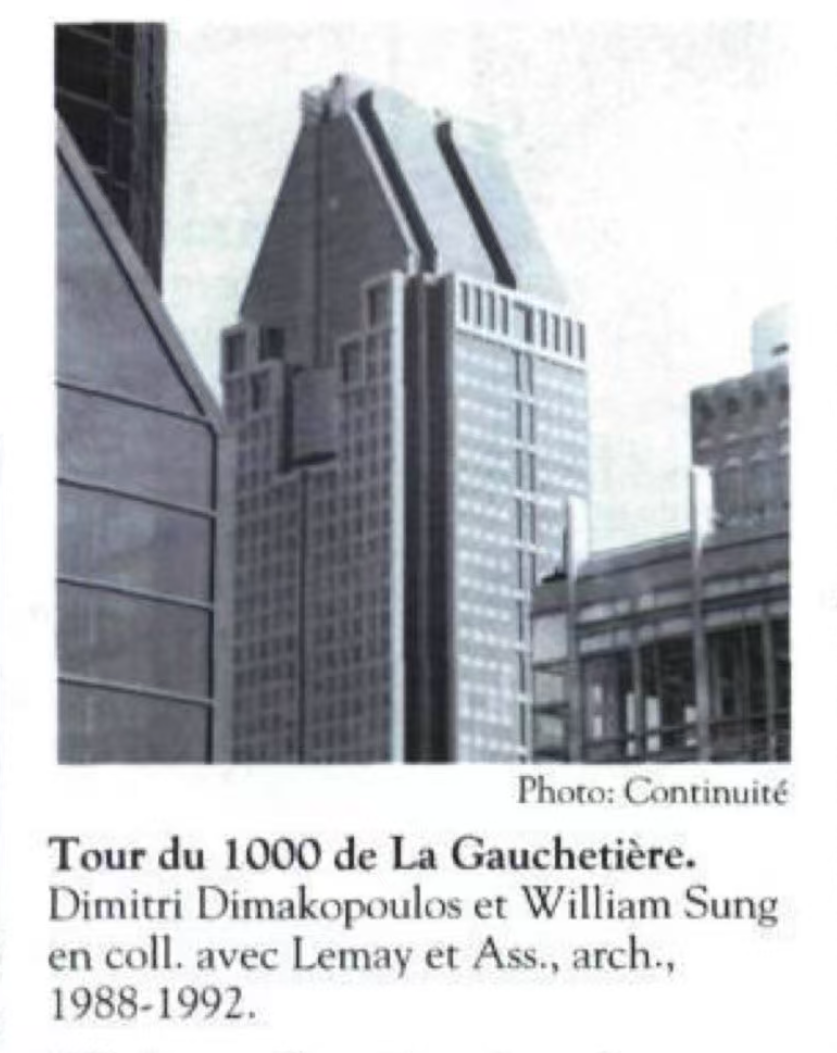
\includegraphics[width=6cm]{!tour_du_1000_deLa_Gauchetiere_250331_thumbnail_picture_(602).png}

\newpage

从小，父母经常给我们灌输的价值观就是：``一定要好好读书，找一个高薪、稳定、不太辛苦的工作，这样年纪大了就能享受轻松的生活了。''因此春节回乡时，亲戚也往往会以收入去评价你。

但随着我工作越久就越来越发现，当收入可以满足家庭的基本需求后，赚钱不再是唯一的追求。其他方面的追求，如工作是否促进自我成长、是否具挑战性和获得满足感等，更为重要。

例如我的二叔William
Sung.，他1933年出生，从小喜欢画画，我还记得看过他的水彩画，很好看。因为他的父母经历过被日军占领3年8个月的日子，都希望子女进政府当公务员，收入稳定有退休金。所以他从香港理工毕业后进政府当卫生检查官。1961年，虽然父母极力反对，他拿着McGill
U的录取信，坐船经日本到加拿大，开始在Montreal读建筑。因为没有父母资助，为节省开支，开始时只能吃罐头、面包，与其他香港同学合租在一间很小的单间。他擅长手工绘制建筑设计图、透视图，在大二开始已经有客户付费请他画图，渐渐有了积蓄，甚至买车，毕业后加入Dimakopoulos
\& Partners，成为合伙人，实现了他的梦想。

所以自己必须有明确清晰的目标，才能不悔此生。企业也类似，所以企业家必须清楚企业的具体标：\\
``5年10年后，希望公司会有什么成就？''

有些企业只有盈利，收入等财务（可量化）目标，但卓越的企业除了这些财务目标以外，更重要有更高的理想和愿景，才能吸引有抱负，有能力的人才加入。（企业的成功还是靠人才。）\\
有些公司为每个岗位设定了KPI，考核结果将直接影响年终奖或晋升。但在与员工的讨论中发现，即使团队成员的KPI全部达标，但整体结果（如成本、质量）却未必理想。所以，如果管理者只追求可量化的指标，而忽视了责任心、团队协作等难以量化的因素，反而会损害整体业务。

例如，某公司每月会选出一位``本月之星''员工，并进行表扬，因缺乏客观的量化指标，竟以员工的打卡时间来衡量。所以KPI或``本月之星''等``激励''措施可能会适得其反。

如果在定期高层会议里，大部分时间都是用于关注各员工的KPI指标是否``高分''，而且没有明确公司愿景，企业就会难以持续健康成长。

所以当 Robert Kaplan与David
Norton在1992年提出平衡计分卡时，商务指标只是4类指标之一，其他还包括：

\begin{itemize}
\tightlist
\item
  从客户视角的指标（客户如何看我们？）
\item
  公司内部业务指标（公司内部卓越之处）
\item
  创新与成长的指标
\end{itemize}


%done-1

\chapter{A27 电话} % Introduction chapter suppressed from the table of contents

\hypertarget{ux66feux7ecfux4fc3ux8fdbux4ea4ux6d41ux7684ux7535ux8bddux73b0ux5728ux5374ux65e5ux76caux6210ux4e3aux4ea4ux6d41ux7684ux969cux788d}{%
\section{曾经促进交流的电话，现在却日益成为交流的障碍}\label{ux66feux7ecfux4fc3ux8fdbux4ea4ux6d41ux7684ux7535ux8bddux73b0ux5728ux5374ux65e5ux76caux6210ux4e3aux4ea4ux6d41ux7684ux969cux788d}}

(56 The telephone, which once facilitated communication, now
increasingly obstructs it.)

\framebox{%
\begin{minipage}[t]{0.97\columnwidth}\raggedright
Prof Ackoff 经验之谈：\\
如今，接电话的人可以这样巧妙地告诉打电话的人不想被联系：先将电话置于等待状态；最后再挂掉。

过去，只需要拨打七位数字即可联系到大多数的人（美国本地电话仅需七位数字）。

如今，电话号码的位数和等待时间成倍增加，远超常人的记忆力和耐心所能承受的范围。

原本希望通过电话找到合适的联系人，却常常因人工生成的电话转接号码无效而徒劳无功。

即便偶尔联系到某人，却往往因为对方没有能力响应需求，也不知应转接何人，又引发一连串的转接，最终以精心设计的``意外''中断告终。

电话曾帮我们大幅减少书面沟通的需求，如今却迫使我们重拾传统的沟通方式。
\strut
\end{minipage}}

\textbf{严重故障需求流程图} （图27）\\
%\href{文件:value_1-3.jpg}{600px}

\includegraphics[width=6cm]{value_1-3.jpg}

\newpage

不知道大家每天会收到多少骚扰电话？通常，我的反应是直接问``哪位？''，确认是陌生人便直接挂断。\\
在教授所处的年代，骚扰电话尚未泛滥，被呼叫者还能礼貌拒绝。\\
如今，我倒有点同情那些被迫拨打骚扰电话的员工，他们每日重复这些工作，想必备受煎熬。问题的根源在于管理层，他们误以为电话促销仍有效，殊不知这种方式不仅效果近乎为零，还损害公司形象。在互联网时代，搜索引擎的功能强大如此，如果产品足够优秀，只需在网站展示并得到用户的点赞，客户自会主动搜索，无需电话推销。\\
正因电话的滥用，人们更渴望免受打扰，可以安静地专注于自己的工作。\\

每次听到``查询余额按1，转账按2，优惠活动按3\ldots{}\ldots{}''这样的自动应答系统录音，我就会直接挂断。经验告诉我，指望这些系统永远无法连通我需要的服务。不少银行、售票等行业普遍采用此类系统一些有经验的客户经理会直接告知正确按键顺序（如1342）或人工客服接入方式，以节省时间。或如何可以直接与人工客服对话，减小对我的耽误。如今，随着科技不断进步，部分公司引入机器人模拟真人对话，但效果未必好。如某售票系统的机器人会热情地问候：``早上好！小倩很高兴为您服务，请问有什么可以帮助您的？''\\
然而，两分钟的``对话''后，系统又提示输入身份证的后四位号码，而我只有港澳通行证号，最终还是无法购票。（但若是与真人通话，整个交易通常在2-3分钟即可完成。）企业误以为机器人（高科技）能提升客户满意度，实则适得其反，客户只会更觉烦躁。所以我总想绕过系统自动应答，直达人工客服，却从未成功破解其设计。\\
在精益价值流培训过程中，我会展示前面的图27，并提问：``如果现在处理存在严重缺陷的流程，从提出申请到解决需要10天。请问有何建议可以缩短时间、减少浪费的？''\\
学员们经过讨论并提交建议后，我接着再问：``是否考虑让用户直接联系开发工程师？''\\
他们又回应：``开发和测试都太忙了，如无客服预先过滤，工程师无法承受这么大的工作量。''\\
接着我分享如下案例：``某公司有800位工程师，在传统客服过滤的模式下，工程部用于处理严重缺陷约占60\%的工作量。变更流程后，通过工程师直接接听客户电话，工作量降至24\%。''
学生觉得不可思议，我接着说：``通过工程师接听客户电话，他们同步提供了客户缺陷与对应的解决办法，并更新到知识库，供客户自查。这不仅将响应时间缩短至原来的三分之一，还让工程师直接收集到用户使用系统过程中遇到的问题，深入了解客户的使用场景，为下一版本的改进提供洞见。''\\
唯一不变的唯有改变。 (The only thing that is constant is change / Change
is the only constant in life)\\
若能跳出思维定式，便能海阔天空，激发无限创意。


%done-1


%\part{团队与自我改善基本功}改善都应从团队开始，并要改善本来的工作习惯的不足，但改变工作习惯并不容易。首章用实例介绍公司团队如何从“破冰”到变革， 到稳定，以及成功要素。

%团队的提升依赖于个人的成长与提升。敏捷开发假定每位成员都具备极高的经验与能力，如果团队成员都是刚毕业的新手，不建议使用敏捷开发。后面第3章介绍提升个人效率的方法。 






\end{document}
